%Fucking left quote symbol ` and not '    

\chapter{Quantum Chromodynamics} \label{ch:qcd}
In 1968 deep inelastic scatterings performed at the Stanford Linear Accelerator Center showed that the proton had internal structure\cite{Riordan1287} called partons at the time.  Within a decade of this discovery the partons were broken into two categories: the mass carrying fermions were known as the quarks and the gauge boson force carriers were called gluons.  The interactions of these two types of particles were described by the quantum field theory known as quantum chromodynamics (QCD) and by the SU(3) symmetry group.  SU(3) guarantees that color charge is conserved and this results in quarks grouping together into `colorless' hadrons.

\subsection{The QCD Lagrangian}
QCD is the strongest of the known fundamental forces.  It is a gauge field theory described by the Lagrangian density

\begin{equation}
{\cal L}=-\frac{1}{4}F^{\alpha}_{\mu\nu}F^{\mu\nu}_{\alpha}
- \alpha_{s} (\bar{q}_{j}\gamma^{\mu}T_{\alpha}q_{j})G_{\alpha}^{\mu}
+ \bar{q}_{j}(i\gamma^{\mu} \partial_{\mu} - m)q_{j}
\label{eq:lagrangian}
\end{equation}

\noindent
where $q$ and $\bar{q}$ represent the color anti-color fields summed over color $j$, $\alpha_{s}$ is the strong coupling strength,$\gamma^{\mu}$ is the Dirac gamma matrix, $G_{\alpha}^{\mu}$ is the gauge field for color \textit{$\alpha$}, is similar in analogy to the \textbf{W} matrix from the electroweak theory.  $F^{\alpha}_{\mu\nu}$ is the field strength tensor and it describes the gluon interactions. The first term of the Lagrangian is the gluon contribution and carries no mass term.  The second term of the Lagrangian describes how quarks and gluons interact with each other. The final term describes quark interactions and the coupling between them and will be explored further in this thesis.

At short distances, less than 0.2 \textit{fm}, the strong coupling constant becomes exceedingly small and second term of the Lagrangian displays an important property known as asymptotic freedom\cite{Wilczek:2005az}. 


\subsection{Scattering and Hard Processes}




\subsection{Factorization}

\subsubsection{Hadronization and Fragmentation}

\subsubsection{Partonic Distribution}


\subsection{Kinematics}\label{sec:kinematics};
Before I give a detailed discussion of the physics and observables in high energy and nuclear physics it would be advantageus to define some terms and go over a few formulas.

In a circular particle accelerator a beam of relativistic particles travels along a beamline.  The coordinates along this beamline are broken into longitudnal and transverse component. The momentum can similarly be described in these coordinates as the longitudnal and transverse momentum, denoted as $\mathbf{p}_{L}$ and $\mathbf{p}_{T}$.  For cylindrical detectors like ALICE\footnote{See Chapter \ref{ch:alice}} it is more advantageous to use a cylindrical coordinate system of with $\theta$ as the polar angle and $\phi$ as the azimuthal angle.  Relativistic particles traveling along the beamline will have 

\begin{equation}
\textit{y} = \frac{1}{2} \ln \frac{E + |\mathbf{p}|}{E - |\mathbf{p}|}
\label{eq:rapidity}
\end{equation}

\begin{equation}
\eta = \frac{1}{2} \ln \frac{|\mathbf{p}| + p_{L}}{|\mathbf{p}| - p_{L}}
\label{eq:psuedo}
\end{equation}

\noindent
Therefore in terms of cartesian coordinates with the x-y plane as the plane transverse to the beamline and the z component as the component along the beam line we can derive the following relationships

\begin{equation}
p_{x} = p_{T} \cos \phi
\label{eq:xcomp}
\end{equation}
\begin{equation}
p_{y} = p_{T} \sin \phi
\label{eq:ycomp}
\end{equation}
\begin{equation}
p_{z} = p_{T} \sinh \eta
\label{eq:zcomp}
\end{equation}

\noindent
The advantage of using the azimuthal angle and psuedorapidity over cylindrical or Cartesian coordinates is that given any two particles, the separation between $R = \sqrt{ (\phi_{i} - \phi_{j})^{2} + (\eta_{i} - \eta_{j})^{2}  } $ is invariant under all Lorentz boosts along the beamline.


\begin{figure}[h]
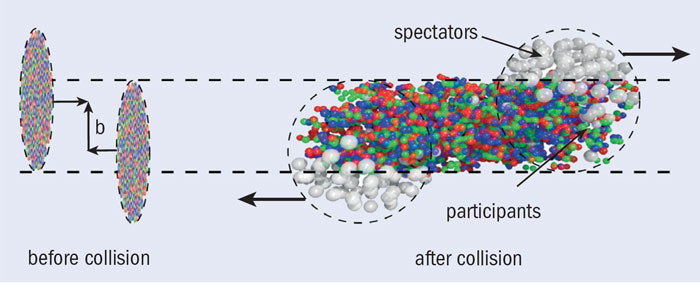
\includegraphics[width=10.0cm]{CCfir5_04_13}
\centering
\caption{Nuclear collison  .}
\label{fig:centrality}
\end{figure}

\noindent
In nuclear collisions the offset between the centers of two nuclei is known as the impact parameter (b) as seen in Figure \ref{fig:centrality}.  Measuring the impact parameter in an experimental setting is non-trivial and model-dependent.  The distribution of nucleons in the nucleus is modeled after a Glauber distribution\cite{Loizides:2016djv}.  The Glauber model predicts that there is a direct correlation between the impact parameter of a nuclear collision and to the inelastic differential cross section ($\sigma_{inel}$)\cite{Miller:2007ri}.


\begin{equation}
c(b) =\frac{ \int_{0}^{b} \frac{d \sigma}{db} db}{ \int_{0}^{\infty} \frac{d \sigma}{db} db} = \frac{1}{\sigma_{inel}} \int_{0}^{b} \frac{d \sigma}{db} db
\label{eq:centrality}
\end{equation}




%JETS
\section{Jets}

Hard probes (large $Q^{2}$ interactions), are produced in the earliest stages of a high energy collision during the largest momentum transfer.  As two highly energetic partons propagate away from one another they will instigate a shower of daughter partons via gluon radiation and the generation of q$\bar{q}$\, pairs.  The clustering of these daughter partons or the final state hadrons they form into is colloquially known as a `jet'.   Jets have been the workhorse for probing QCD phenomena by both theroetically and experimentally for over 30 years.  

\subsection{Jet Finding Algorithms}
Although, it may simple to have a conceptual grasp of what a jet `is' there is no unambiguous definition, both experimentally and theoretically, for how to define a jet.  This is due to the fragmentation process by which partons form into their final state hadrons is not calculable pertubatively.  The earliest jet measurements used multiple definitions which complicated comparisons between experiments and theoretical calculations.  In 1990, the Snowmass Accord\cite{Huth:217490} was held in order to standardized the definition of a jet between experimentalists and theroeticans.  The agreement maintained that any algorithm that clusters particles into a jet must be both infrared and collinear safe (IRC).  If a high-momentum parton radiates a soft gluon tis emisson should not affect the 

Although there are a number of jet finding algorithams available, I will only focus on algorithams that are both collinear and infrared safe.   




%\subsection{Jets in Proton Collisions}

%\subsection{Jets in Heavy Ion Collisions}

%QGP
\section{The Quark-Gluon Plasma}

\subsection{Asymptotic Freedom and the Perfect Fluid}

\subsubsection{Hydrodynamics}
The conservation laws for a relativistic fluid conserve the charge current and energy-momentum tensor of the expanding fluid such that:

\begin{equation}
\partial_{\mu} N_{\textit{i}}^{\mu} = 0
\label{eq:hydrochrg}
\end{equation}

\begin{equation}
\partial_{\mu} T^{\mu \nu} = 0
\label{eq:hydroenrgy}
\end{equation}

\subsection{Energy Loss in a Colored Medium}

\subsection{The Nuclear Modification Factor}

\subsection{Nuclear Collisions}

%\subsection{Jet Results from Nuclear Collisions}

\section{QGP in Proton-Proton Collisions?}
As previoulsy stated a QGP is believed to be absent in proton-proton collisions, thus any signature of a QGP should likewise be absent.  One way of quantifying the presence of the QGP is via the Bjorken energy density.  

\begin{equation}
\varepsilon = \frac{1}{\tau A} \frac{dE_{T}}{d \eta}
\label{eq:bjorkenEt}
\end{equation}

\noindent
where A is the transverse area of the nuclei, $\tau$ is the proper time, and $dE_{T}/d \eta$ is the transverse energy per unit psuedorapidity.  It can be shown that  the 150 MeV critical temperature need for the phase transition to the QGP corresponds to ~ $1 - 3 GeV/fm^{3}$ energy density.  The quantity $dE_{T}/d \eta$ can be related to the mean transverse momentum $<p_{T}>$ and particle multiplictiy\footnote{Multiplicity is defined as the number of particles per event} per unity psuedorapidity as:

\begin{equation}
\frac{dE_{t}}{d \eta}  \approx  <p_{T}> \frac{dN}{d\eta}
\label{eq:Et}
\end{equation}

where $ <p_{T} >$ is the mean transverse momentum and $dN/d\eta$ is the particle multiplicity per unit psuedorapidity.
This suggest that in very high multiplicity proton-proton events signatures of the QGP may be present.  This is one of the most active and newest areas of research in heavy ion physics.  